%\section{Proposed Approach}

\begin{frame}{System Architecture}
\begin{minipage}[t]{0.6\linewidth}
\centering 
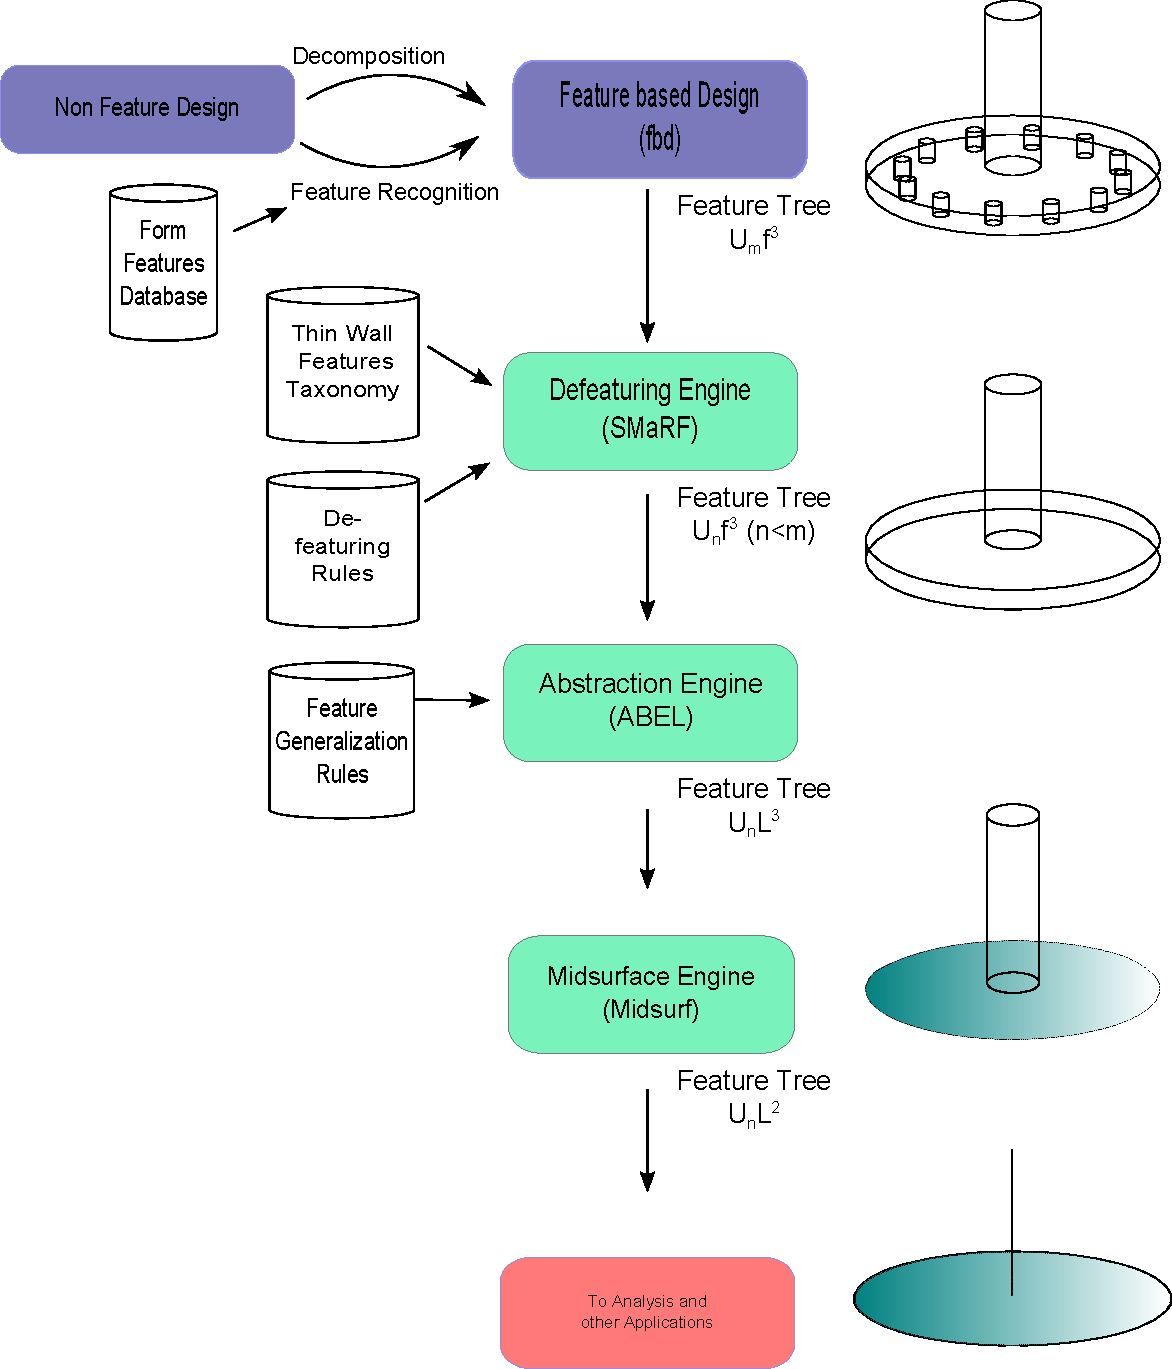
\includegraphics[width=\linewidth]{../Common/images/SystemArchitecture1.pdf}
\end{minipage}
\note{
\begin{itemize}[noitemsep,topsep=2pt,parsep=2pt,partopsep=2pt]
\item Input is a feature-based CAD model represented by  ($\cup_uf^3$), where $\cup$ denotes a collection of $u$ features ($f$)  having dimensionality $3$ (solids).
\item \textbf{Defeaturing Engine (SMaRF)}\cite{YogeshCADConf2015}: The model is de-featured to the remove small irrelevant features, there by, reducing their count to $v$. So the model now becomes ($\cup_vf^3, u \leq v$).
\item \textbf{Abstraction Engine ($\mathcal{ABLE}$)}\cite{YogeshIITG2014}: Each form feature is abstracted in the form of ``Loft or Sweep'' representation containing the profile $p$, guide curve $g$, along with the internal boolean $b$. The model then becomes ($\cup_vL^3$).
\item \textbf{Midsurface Engine (Midsurf)}: All such abstracted feature bodies undergo cellular decomposition (fbCD) and the output is a list of non-volumetrically-overlapping cell-bodies having Sweep-based feature owners. This module is elaborated in the following sections.
\end{itemize}
}
\end{frame}

\begin{frame}{Face Pairs Detection Problem}
\begin{itemize}[noitemsep,label=\textbullet,topsep=2pt,parsep=2pt,partopsep=2pt]
\item Face pairs, in a way, decompose the whole shape into sub-volumes. 
\item Each sub-volume, creates its own midsurface patch. 
\item The main challenge in using the features is their variety.
\item Convert to $\mathcal{ABLE}$: ``Sweep'' with a profile and  a guide curve.
\item Sweeping the profile upto half of the guide curve, or 
\item By sweeping the midcurve of the profile by a full guide curve. 
\item Using this, the necessity of detecting face pairs can be avoided.
\end{itemize}
\begin{center}
\begin{tabular}{c c c}
\raisebox{-.9\height}{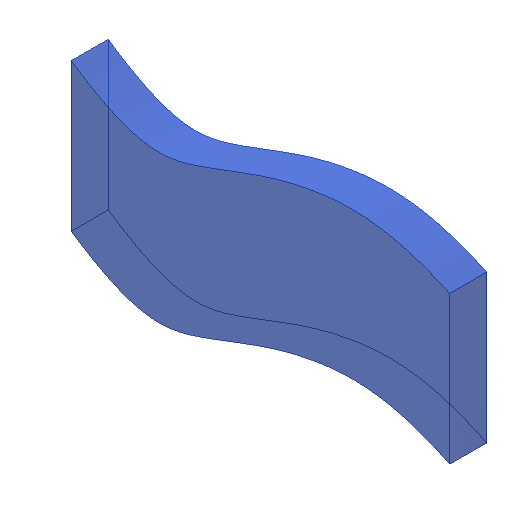
\includegraphics[width=0.2\linewidth]{../Common/images/ThickThinProfilePart}} & 

\raisebox{-.9\height}{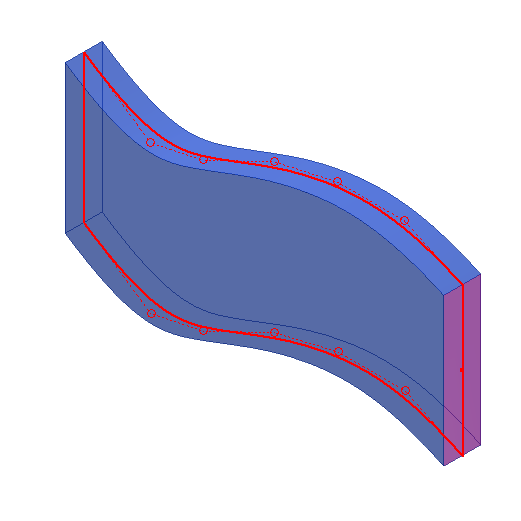
\includegraphics[width=0.2\linewidth]{../Common/images/ThinProfileMidsurf}} & 

\raisebox{-.9\height}{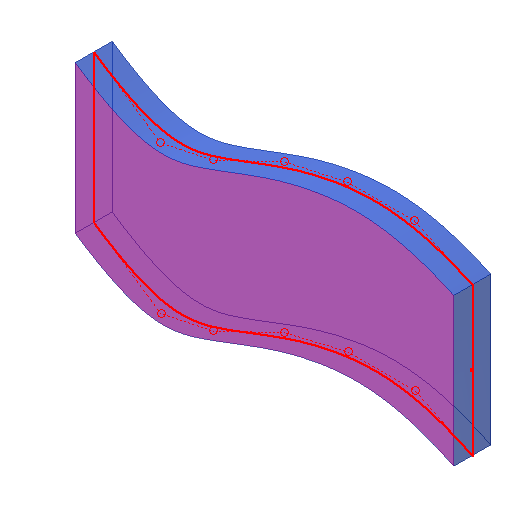
\includegraphics[width=0.2\linewidth]{../Common/images/ThickProfileMidsurf}} \\


Shape  & Thin Profile & Thick Profile \\ 
\end{tabular}\end{center}
\end{frame}

\begin{frame}{Face Pair Interaction Problem}
\begin{itemize}[noitemsep,label=\textbullet,topsep=2pt,parsep=2pt,partopsep=2pt]
\item Critical to ``joining'' is to know how the features interact. 
\item No framework for all interaction types, so, no unified logic \cite{Stolt2006}.
\item A large variety is possible, as Aligned, L, T, Overlap and Crossing.
\item

\begin{tabular}{c c c}
\raisebox{-.9\height}{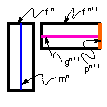
\includegraphics[width=0.25\linewidth]{../Common/images/FeatureInteractionStageN.pdf}} & 

\raisebox{-.9\height}{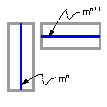
\includegraphics[width=0.25\linewidth]{../Common/images/MidsurfInteractionStageN.pdf}} & 

\raisebox{-.9\height}{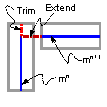
\includegraphics[width=0.25\linewidth]{../Common/images/MidsurfExpectationStageN.pdf}} \\


%Feature Interaction  & Midsurface Interaction & Midsurface Processing\\ 
\end{tabular}
\item Note: Using simple diagrams but applicable to others as well
\item For each, 3 variations of the profile and guide curve locations.
\end{itemize}
\end{frame}



\begin{frame}{Interaction types}
\resizebox{0.45\linewidth}{!}{
\centering
\begin{tabular}[h]{@{}p{0.12\linewidth} p{0.3\linewidth}  p{0.3\linewidth}  p{0.3\linewidth} @{}} \toprule
{\bf Type} & {\bf Interaction}  & {\bf Midsurface} & {\bf Joining} \\ \midrule  
L type/ End  &
\adjustbox{valign=t}{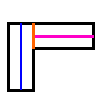
\includegraphics[width=\linewidth]{../Common/images/pogtlei.pdf}}  &  
\adjustbox{valign=t}{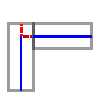
\includegraphics[width=\linewidth]{../Common/images/pogtlem.pdf}} &  
Guide curve needs to be extended in the other direction till the existing midsurface. Trim and remove the extra patches of the existing midsurface. 
\\ \midrule

T type/ Middle  &
\adjustbox{valign=t}{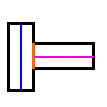
\includegraphics[width=\linewidth]{../Common/images/pogtlmi.pdf}}  &  
\adjustbox{valign=t}{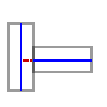
\includegraphics[width=\linewidth]{../Common/images/pogtlmm.pdf}} &  
Guide curve needs to be extended in the other direction till the existing midsurface. Do not remove any patch from the existing midsurface. 
\\ \midrule

X type/ Crossing  &
\adjustbox{valign=t}{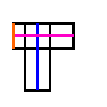
\includegraphics[width=\linewidth]{../Common/images/pfgclei.pdf}}  &  
\adjustbox{valign=t}{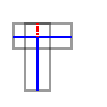
\includegraphics[width=\linewidth]{../Common/images/pfgclem.pdf}} &  
Guide curve does not need to be extended. Remove the extra patch of the existing midsurface.
\\ \midrule

Align  &
\adjustbox{valign=t}{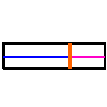
\includegraphics[width=\linewidth]{../Common/images/pogtlai.pdf}}  &  
\adjustbox{valign=t}{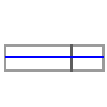
\includegraphics[width=\linewidth]{../Common/images/pogtlam.pdf}} &  
 No adjustment needed	
\\ \midrule

Overlap  &
\adjustbox{valign=t}{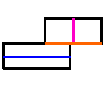
\includegraphics[width=\linewidth]{../Common/images/pogflpi.pdf}}  &  
\adjustbox{valign=t}{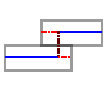
\includegraphics[width=\linewidth]{../Common/images/pogflpm.pdf}} &  
 Trim the extra patches from the new as well as existing midsurfaces. Join the new edges with an additional patch.
\\
\bottomrule
\end{tabular}
}
\end{frame}

\begin{frame}{Cellular Decomposition}
\begin{itemize}[noitemsep,label=\textbullet,topsep=2pt,parsep=2pt,partopsep=2pt]
\item Clear that the numbers of interactions are too many. 
\item Developing logic for each of these cases can be a tedious task. 
\item Desirable to provide a uniform logic that can take care of all or most of the cases. 
\item All-encompassing scheme is possible with cellular representation.
\end{itemize}
\begin{center}
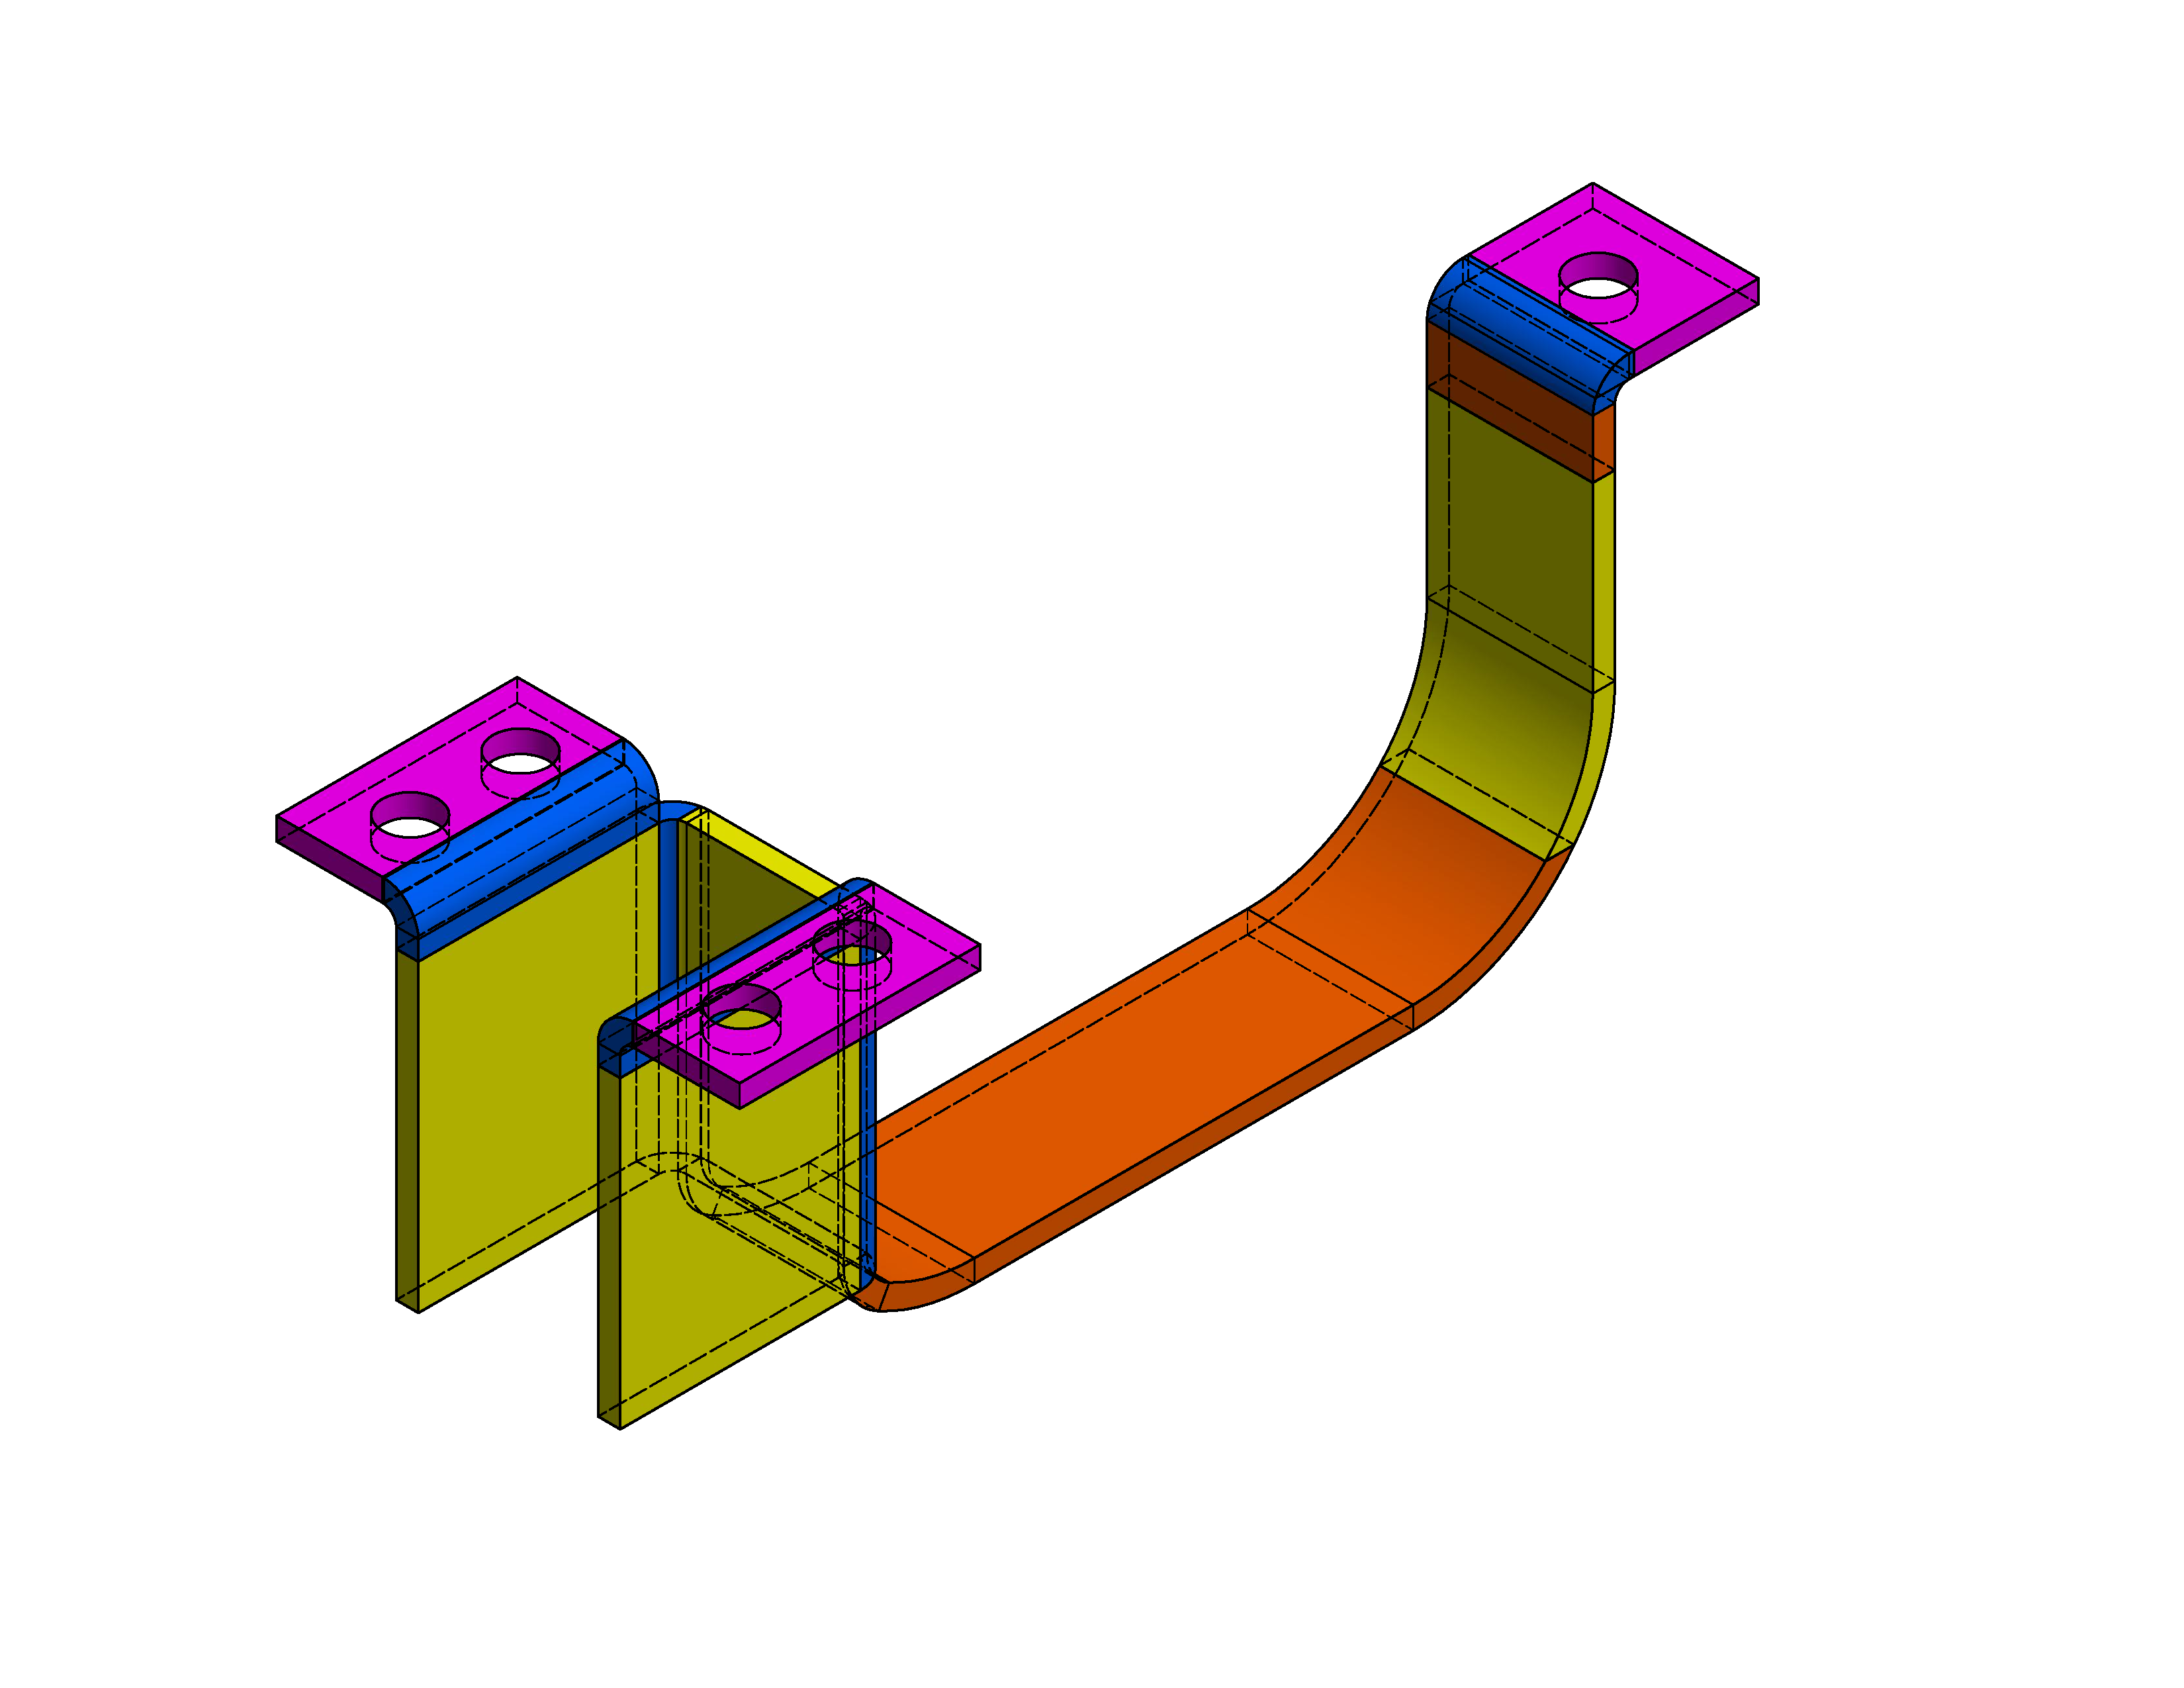
\includegraphics[width=0.55\linewidth]{../Common/images/VolDecomp1.pdf}
\end{center}
\end{frame}

\begin{frame}{Overall Algorithm}
\begin{itemize}[noitemsep,label=\textbullet,topsep=2pt,parsep=2pt,partopsep=2pt]
\item Input is a feature-based design (fbd) CAD model 
\item Fbd is decomposed into cells-bodies, with the assigned feature owners. Cell-bodies do not overlap volumetrically, but may overlap at faces, fully.
\item An adjacency-graph is formed with the nodes ($n$) representing the cell-bodies. For each such face-overlap, a corresponding edge ($e$) is created in the graph. An edge $E$ has two $n$s attached on either end.  
\item Cells are classified into solid cells ($sCell$) and interface cells ($iCell$).  The commonly shared cells are marked as interface cells ($iCell$) and the others as solid cells ($sCell$)
\vspace{-4mm}
\begin{figure}[!h]
\centering     %%% not \center
\subfloat[Decomposition]{\label{fig_interaction}\includegraphics[width=0.6\linewidth]{../Common/images/CellDecompExample}}
\subfloat[Graph]{\label{fig_patches}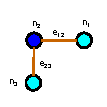
\includegraphics[width=0.25\linewidth]{../Common/images/FeatureInteractionGraph.pdf}}
\end{figure}

\end{itemize}
\end{frame}


\begin{frame}{Overall Algorithm cont...}
\begin{itemize}[noitemsep,label=\textbullet,topsep=2pt,parsep=2pt,partopsep=2pt]
\item For each $sCell$ the midsurface is computed

\vspace{-3mm}

	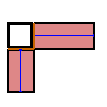
\includegraphics[width=0.25\linewidth]{../Common/images/MidsurfPatches.pdf}	
	
\vspace{-3mm}	

\item As the owner feature is represented by ``Sweep/Loft'', extract the profile $p$) and guide curve ($g$).
\item The profile $p$ is considered thin if it's size far less than the size of the guide curve $g$.  Threshold value based on the experimentation is used.
	\item If the profile $p$ is thin: A midcurve ($m^1$) is computed from $p$, $m^1$ is swept using guide curve $g$ to generated midsurface patch $m^2$.
	\item If the profile $p$ is thick: $p$ is offset by half of $g$ so as to lie midway. 
\end{itemize}
\end{frame}

\begin{frame}{Overall Algorithm cont...}
\begin{itemize}[noitemsep,label=\textbullet,topsep=2pt,parsep=2pt,partopsep=2pt]
\item  For each $iCell$ the midsurface extensions are computed
\vspace{-2mm}
	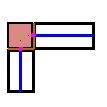
\includegraphics[width=0.25\linewidth]{../Common/images/MidsurfJoining.pdf}	
\vspace{-2mm}	
\item Each $iCell$ is connected with other cells via edges $e$(s). 
\item For each $e$, there are two nodes- one is ``self'' $iCell$ and the second   one is called the ``other node''. 
\item Depending on whether the ``other node'' is $sCell$ or $iCell$, the logic differs. 
\item If the ``other node'' is $sCell$, Extend  up to $iCell$'s centroid
\item  If the ``other node'' is a $iCell$, an extra patch is needed between the centroids of the two $iCell$s.
\end{itemize}
\end{frame}
